\newcommand{\SK}[1]{{\small\textcolor{blue}{[NOTE: #1]}}}
%There are some concepts that the reader should be familiarised with in order to fully understand the work described in the following chapters. These concepts are briefly explained in this chapter in order to contextualize and help the reader understand the rest of this writing.
% bit of the development history of machine translation.
This chapter walks through the background to understand our research. In Section \ref{section:MT}, we explain what is machine translation (MT), and its evolution by covering several MT approaches in the past. We explain what is NMT and one of the state of the art architectures in Section~\ref{section:NMT}. In Section~\ref{section:transfer_learning}, one of the common methods for improving NMT performance, domain adaptation will be covered. For training MT systems, assessment of system output is essential. Section~\ref{section:evaluation_metrics} will describe automatic evaluation metric of MT and especially, BLEU. Training such NMT models are complex and can confront overfitting issues. In Section~\ref{section:Regularization}, we introduce multiple regularization methods to prevent overfitting. Lastly, we conduct a short research review related to using confidential data in NMT. 


\section{Machine Translation}\label{section:MT}

Machine translation (MT) is a field of research in natural language processing (NLP), the task of converting an input consisting of a sequence of words in a source language into a sequence of words in a target language. %Translation is a difficult task that requires a long training period for humans, and hence, is more challenging for machines. 
This can be formulated as Equation~\ref{equ:MT}. %\parencite{eisenstein2019introduction}
%$\hat{s^{(t)}} = argmax\Psi(w^{(s)}, w^{(t)}) $
\begin{equation}
    \hat{\textbf{t}} = \argmax_{\textbf{t}}\Psi(\textbf{s}, \textbf{t})\
    \label{equ:MT}
\end{equation}

where $\textbf{s}$ and $\textbf{t}$ represent sentences of source and target languages, receptively. $\hat{\textbf{s}}$ is generated translation and $\Psi$ is a scoring function. In general, MT models consist of decoding $\textbf{s}$ into $\textbf{t}$ and learning algorithms for parameters of $\Psi$.

% Machine translation is originated in the 1950s and has since developed a number of different approaches.

\subsection{Quick MT history}

MT began around the 1950s and has since developed numerous approaches. The early MT models were mostly about a direct word to word translation based on bilingual dictionaries, rule-based MT (RBMT). Linguistic experts created a large set of rules for each language pair. Based on the built-in rules, the MT system translates directly source words to corresponding target words. However, RBMT required too many linguistic rules that were manually created and adapting new rules was complicated~\parencite{lagarda-etal-2009-statistical}.
Therefore, to reduce linguistic information and human involvement in building rules, the desire to teach MT systems through examples began to arise naturally.

In the 1990s, \cite{brown-etal-1993-mathematics} proposed corpus-based approaches as a beginning of modern statistical MT (SMT): a parallel corpus was needed with minimum linguistic information to train MT systems. Finally, \cite{berger-etal-1994-candide} introduced the first SMT model without any linguistic rules. The main idea of SMT is to learn a probabilistic model from samples of parallel corpora. Various models have been proposed for SMT, in particular the phrase-based SMT (PBSMT) model \parencite{koehn-etal-2003-statistical} has been widely used.

%While statistical machine translation (SMT) has been successfully deployed in many commercial systems, it does not work very well and suffers from the following two major drawbacks. First, translation decisions are locally determined as we translate phrase-by-phrase and long-distance dependencies are often ignored. More problematically, the entire MT pipeline is becoming increasingly complex as more and more features are added to the log- linear framework such as in recent MT systems.

\section{Neural Machine Translation}\label{section:NMT}

\begin{figure}[H]
    \centering
    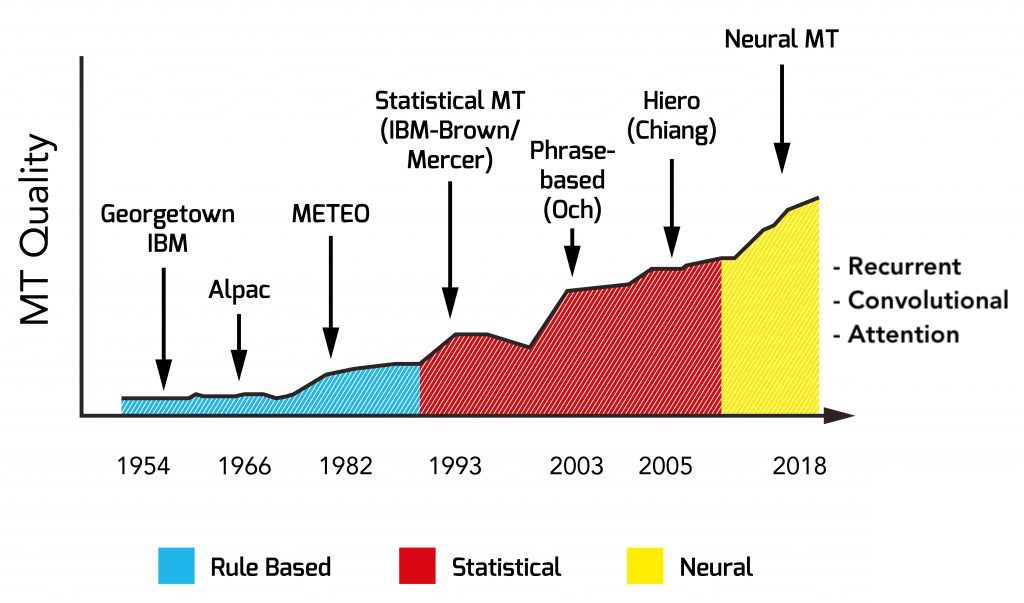
\includegraphics[scale=0.30]{images/A-brief-history-of-MT.jpeg}
    \caption{The improvement of MT quality: Since the 1950s, the MT systems have been evolved through multiple approaches. Currently, NMT dominates in MT~\parencite{iconictranslation}}
    \label{fig:brief_history}
\end{figure}

Advances in neural network based models have led to astonishing improvements in MT~\parencite{sutskever2014sequence, bahdanau2014neural, vaswani2017attention}. As Figure~\ref{fig:brief_history} shows, NMT represent the current state-of-the-art in this task~\parencite{hassan2018achieving}.One of the strengths of NMT is unlike traditional SMT models, it can directly learn the mapping from the input sequence to the corresponding output sequence in an end-to-end manner. This can exploit bigger context information than SMT models, and this can be possible because of encoder-decoder architecture.

\begin{figure}[ht]
    \centering
    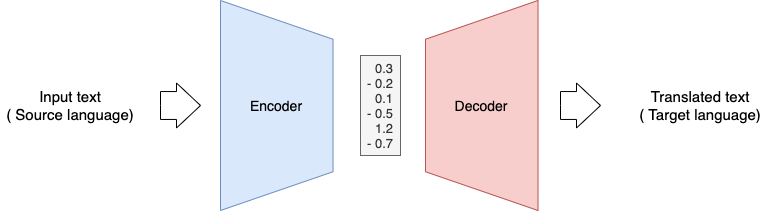
\includegraphics[scale=0.6]{images/encoder-decoder.png}
    \caption{Encoder-Decoder architecture for NMT. The model builds a fixed size vector representation with an input sequence. The vector is generated into the output sequence by the decoder.  }
    \label{fig:encoder_decoder}
\end{figure}

\subsection{Encoder-Decoder architecture}

NMT systems are based on the \textit{encoder-decoder} architecture~\parencite{sutskever2014sequence} which consists of the encoder and the decoder. The encoder network receives an input sentence and converts it into a representation in a fixed-sized vector, so called context vector. This context vector contains all the valuable features and information of the input sequence. Then, the decoder network converts the vector into a sequence output in the target language. To do so, the decoder generates the output sentence word by word. The encoder and decoder networks are trained in end-to-end manner. This whole process of an encoder-decoder architecture for NMT is illustrated in Figure\ref{fig:encoder_decoder}. 

In the decoding process, the decoder network aims to choose the most likely output sequence from the target vocabulary. To search for the most proper tokens, various decoding algorithms have been proposed. Currently, beam search is widely used in state-of-the-art NMT systems. Instead of immediately selecting the word with the highest probability as the next word, beam search generates sentences by selecting words with high probability in the second and third (range is determined by beam size). It then calculates the sum of the probabilities of the candidate sentences, and generates the highest-scoring, 'best' output sentences.


\subsection{Attention mechanism}


In the previous Section, the encoder compresses an input sequence into a single fixed-size vector representation called a context vector, and the decoder converts an output sequence from it. Although encoder-decoder architecture is effective, it has problems with long sequences. Since the encoder packs all the information and features into one fixed-size vector, the problem of information loss occurs.
This leads to the decrease of translation quality in long input sentences.

As a solution, \cite{bahdanau2014neural} introduced the attention mechanism. The main idea of attention is that at every time step when the decoder predicts the output word, the entire input sequence at the encoder is referred to once again. However, instead of referring to the whole input sentence with the same importance, some input words more related to the output word predicted at that time step are received more attention. In other words, with the attention mechanism, we can discover which input word of the encoder is the most related to the decoder output at a specific time step. 

% This is described as Equations:

% \begin{equation}
%     Attention(Q, K, V) = softmax\left(\frac{QK^T}{d_k}\right) &  \text{Attention Value,} \\
% \end{equation}

% where the attention can be mapped with query ($Q$), key (K), and value (V). 


% The core idea of the attention mechanism is to make the model 'focus on only the important parts'. 
% Use the attention distribution to take a weighted sum of the encoder hidden states.\\
% The attention output mostly contains information from the hidden states that received high attention.\\
% Attention : Given a set of vector values, and a vector query, attention is a technique to compute a weighted sum of the values, dependent on the query.
% The encoder-decoder architecture with attention mechanism has become the standard approach in MT. 

\subsection{Transformers}

\begin{figure}
    \centering
    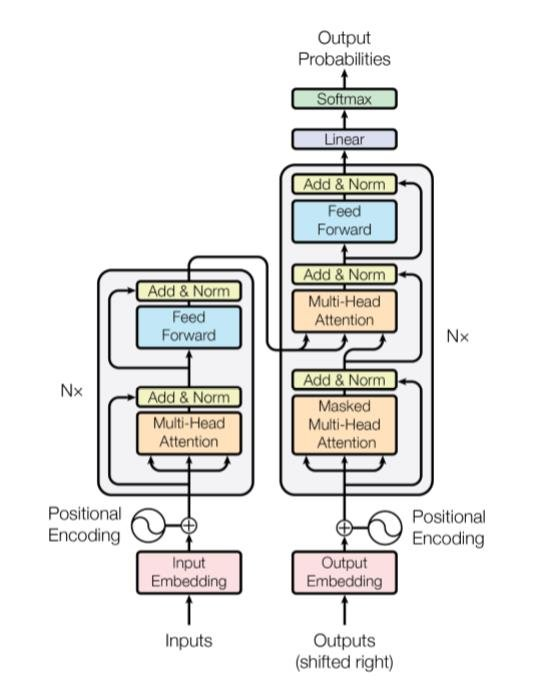
\includegraphics[]{images/The-transformer-model-from-Attention-is-all-you-need-Viswani-et-al.png}
    \caption{The Transformer architecture~\parencite[]{\parencite{vaswani2017attention}} }
    \label{fig:transformer}
\end{figure}
Current state-of-the-art NMT architecture is Transformer architecture~\parencite{vaswani2017attention}. This architecture does not use the recurrent layers commonly used in the encoder-decoder architectures. The transformer uses multi-head self-attention to reduce sequential computation, making more parallelizable while at the same time modelling more inter-word dependencies. This allows the model to train faster. Figure~\ref{fig:transformer} describes the architecture of the transformer. 

Although the transformer does not use a recurrent neural network (RNN), it maintains an encoder-decoder structure. In the traditional encoder-decoder structure, each RNN in the encoder and decoder had t time-steps, but instead of it, in the transformer, the encoder and decoder are N units.

% \subsection{Difficulties of NMT}

% - Low-resource language pairs\\
% - Out-of-vocabulary words\\
% - Domain mismatch between train and test data\\
% - Maintaining context over longer text

%\paragraph{Byte-Pair Encoding}
% \parencite[]{sennrich-etal-2016-neural}


\begin{figure}[hb!]
    \centering
    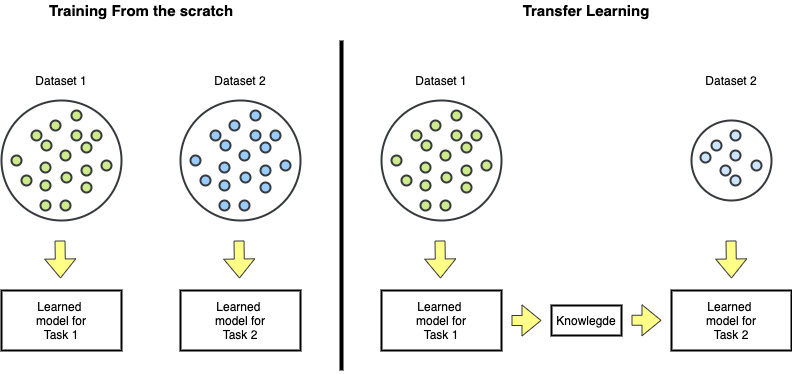
\includegraphics[scale=0.50]{images/transfer_learning.png}
    \caption{The comparison of transfer learning with traditional learning, where start training from scratch.}
    \label{fig:transfer_learning}
\end{figure}

\section{Domain Adaptation for NMT}\label{section:transfer_learning}

Deep learning approaches require huge amount of dataset but in practice, data scarcity issues are common. To tackle this problem, transfer learning is widely used. As Figure~\ref{fig:transfer_learning} describes, transfer learning exploits the knowledge obtained from the previous related learning to the next task. Domain adaptation is a related concept of transfer learning where the task remains the same but the domains are different. However, there seems to be some disagreement among researchers about the definition of transfer learning and domain adaptation. It causes, throughout the literature about them, there are several terminology inconsistencies. In this thesis, we consider domain adaptation is a part of transfer learning.

Domain adaptation is often applied in NMT systems where the target domain data is low resource. There are various methods for domain adaption for NMT, and a comprehensive review of the possible techniques are introduced by \cite[]{chu-wang-2018-survey}. This can be categorised into two groups as Figure~\ref{fig:domain_adaptation_chart} represents: data and model centric. 

Fine-tuning is the conventional way for domain adaptation for NMT~\parencite{luong2015stanford, sennrich-etal-2016-improving}. Fine-Tuning is applied in the scenario where the a NMT system is pre-trained on a rich parallel out-domain data. The NMT parameters are optimised by a much smaller target domain data during fine-tuning.

\begin{figure}[H]
    \centering
    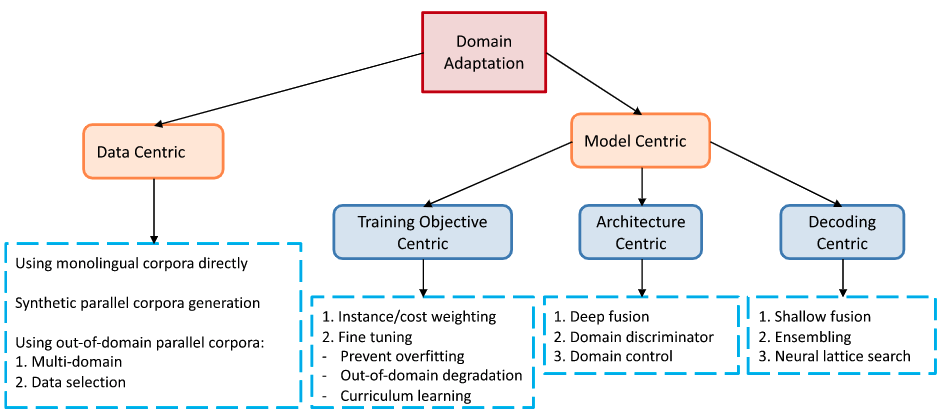
\includegraphics[scale=0.48]{images/domain_adaptation_chart.png}
    \caption{Overview of domain adaptation for NMT~\parencite[]{\parencite{chu-wang-2018-survey}.}}
    \label{fig:domain_adaptation_chart}
\end{figure}

%Domain adaptation means a NMT system is pre-trained on parallel out-of-domain data and then fine-tuned with in-domain sentence pairs. This is so-called fine-tuning. During fine-tuning the NMT systems learn new terminology and sentence structures, resulting in significantly improved performance on the in-domain test set.


\section{Automatic Evaluation Metric}
%by improving translation quality, as measured mainly by automatic evaluation metrics
%Why and how metric is used for MT evaluation
%Besides evaluation, there is also a need for analyzing MT outputs. We recommend the following tools for evaluating and analyzing MT output.
Automated MT quality evaluation metrics are an indispensable part of the MT research area for verifying and analysing the efficiency of MT systems. Even if human translation evaluation is accurate and extensive, it is time-consuming, expensive, language-dependent and inherently subjective. Here, therefore, the need for automatic MT evaluation metrics arises. It provides a rapid, objective and consistent assessment of translation at a low price. The main idea of automatic evaluation metric is to measure how similar the model output (hypotheses text) is to a professional human translation (reference text) using statistical metrics. Multiple automatic methods of MT have been proposed.
%Even if the task of MT is a likelihood-based task maximising the probability of source and target sentences, the evaluation of MT systems examine adequacy, fluency, and fidelity of the translations.
%how to obtain automatic metrics that correlate well with human judgments about the quality of a given translation

\subsection{BLEU}\label{section:evaluation_metrics}

The \textbf{B}i\textbf{L}ingual \textbf{E}valuation \textbf{U}nderstudy (Papineni et al., 2002) (BLEU) method is the current standard for automatic evaluation metric in MT translations. To compute the BLEU score of the generated translations, count the number of N-grams\footnote{The size of N-gram can be from 1 to 4, and in general, size 4 is common. } of overlapping system translations in the reference. BLEU is an N-gram precision metric that measures how close the system output is to a human translation and the precision score is defined as Equation \ref{eq:BLEU_1}.

\begin{equation}
    p_n = \frac{\text{Number of overlapping N-grams in system output and reference}}{\text{Number of N-grams in system output}}
    \label{eq:BLEU_1}
\end{equation}

\begin{equation}
    BP = \begin{cases} 
      1 & \text{if c > r} \\
      e^{(1-r/c)} & \text{if c} \leq \text{r ,} \\
    \end{cases}
    \label{eq:BLEU_2}
\end{equation}

\begin{equation}
   BLEU = BP \cdot exp \left(\displaystyle\sum_{n=1}^{N}w_n log(p_n) \right)
    \label{eq:BLEU_3}
\end{equation}

However, precision-oriented metrics are biased to generate short outputs that only consist of high confident N-grams. To prevent this, a \textbf{brevity penalty} is applied to penalise the BLEU score if the output is shorter than the reference. Equation~\ref{eq:BLEU_2} shows the calculation of brevity penalty in BLEU: $c$ and $r$represent the length of system output and reference, respectively. Finally, the BLEU score is defined in Equation~\ref{eq:BLEU_3} where commonly $N = 4$ and $w_n = \frac{1}{N}$. The BLUE scores range from 0 to 100 and the higher score represents the better translation: Figure~\ref{fig:bleu_google} shows the interpretation of the BLUE scores by \textsc{Google}. 

\begin{figure}[h!]
    \centering
    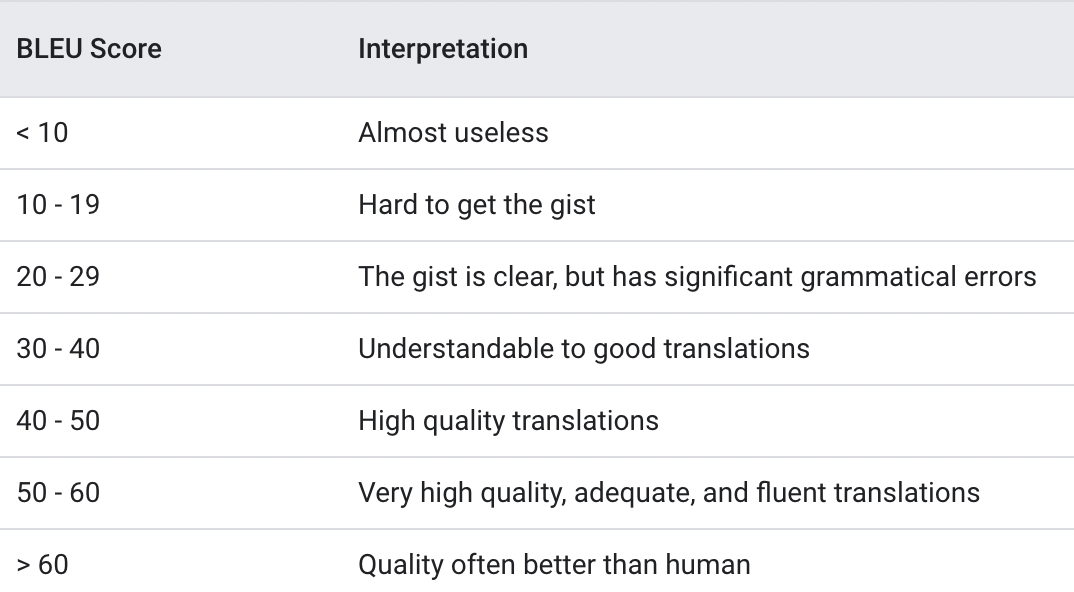
\includegraphics[scale=0.5]{images/BLEU_google.png}
    \caption{Interpretation of BLEU score from Google~\protect\footnotemark}
    \label{fig:bleu_google}
\end{figure}
\footnotetext{This chart is from \url{https://cloud.google.com/translate/automl/docs/evaluate}}

\section{Regularization Techniques for fine-tuning}\label{section:Regularization}%%%%%%%%

Neural network training often runs into the problem of overfitting, where the model performs exceptionally well on the training data but cannot predict the test data. In particular, the overfitting problem can easily arise in scenarios where large, high-performance pre-trained models are used for fine-tuning on typically small in-domain datasets~\parencite{geman1992neural}. This is because neural networks cannot generalize to the unseen data, while decreasing the error on training data. To tackle this problem, various regularization methods are often applied that modify the learning algorithm for better generalisation of the model. In this section, we explain early stopping, dropout and weight decay.

%\cite{miceli-barone-etal-2017-regularization} suggested several regularization techniques to prevent overfitting during fine-tuning, especially for NMT models: To tackle this problem, various regularization methods which modify  the learning algorithms for better generalisation of the model are often applied.
\subsection{Early stopping}\label{chapter:early_stopping}

\begin{figure}[ht]
    \centering
    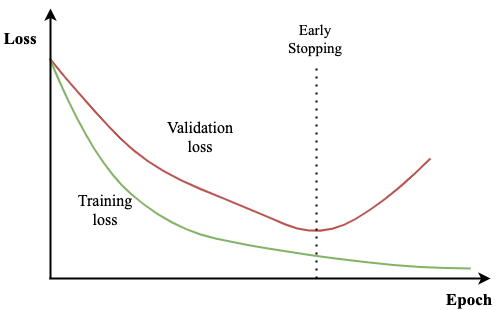
\includegraphics[scale=0.53]{images/early_stopping.png}
    \caption{Early stopping: Learning curves describes how training and validation losses change over epochs. At a certain point, validation loss goes up whereas training loss keeps decreasing.}
    \label{fig:Early stopping}
\end{figure}

When training a neural network with an iterative method, the training error decreases steadily, while the error on unseen examples (i.e. test or validation set) can worsen. To avoid the overfitting problem, early stopping is the most common regularization method in deep learning because it is simple but very effective. As Figure~\ref{fig:Early stopping} illustrates, early stopping aims to stop training the model when the validation set error reaches the lowest point. While training a model it is evaluated on the validation set after each epoch of training. The parameter settings are saved and training continues while this validation set error is progressively improved. Training terminates when the error on the validation set becomes worse or cannot progress compared to the previous validation error. Here, the error in the validation assumes the generalisation error.  

Early stopping requires a validation set. To obtain it, the training data is split into a smaller training set and a validation set. In a scenario where cannot afford large in-domain data, some in-domain data will not be available for training. However, according to the results of \cite{miceli-barone-etal-2017-regularization}, early stopping is a powerful way to prevent overfitting, despite the disadvantage of reducing the training data.

\subsection{Dropout}


%During training time, dropout randomly sets node values to zero. 
Dropout~\parencite{srivastava2014dropout} has been widely used against overfitting problem in deep learning. As Figure~\ref{fig:Early stopping} illustrates, the main idea of dropout is to randomly ''drop out'' units and their corresponding connections while training the neural network. This alleviates over \textit{co-adaptation} of units in the network. In neural network, co-adaptation refers to units in a neural networks have highly correlated to each other. This may cause overfitting since these highly co-adapting units cannot detect features independently and difficult to generalise to unseen data. Thus, to prevent co-adaptation, dropout makes units unreliable to others by killing random units. During training, the network randomly sampled with a dropout probability $p$ and only the sub-networks are trained. Afterwards, at test time, the neural network does not use dropout, and the units of the network have smaller weights than trained ones. In other words, each unit during testing is always used and the weights are multiplied by dropout probability $p$. This allows the network to easily estimate averaging the prediction of all sub-networks.

\begin{figure}[ht]
    \centering
    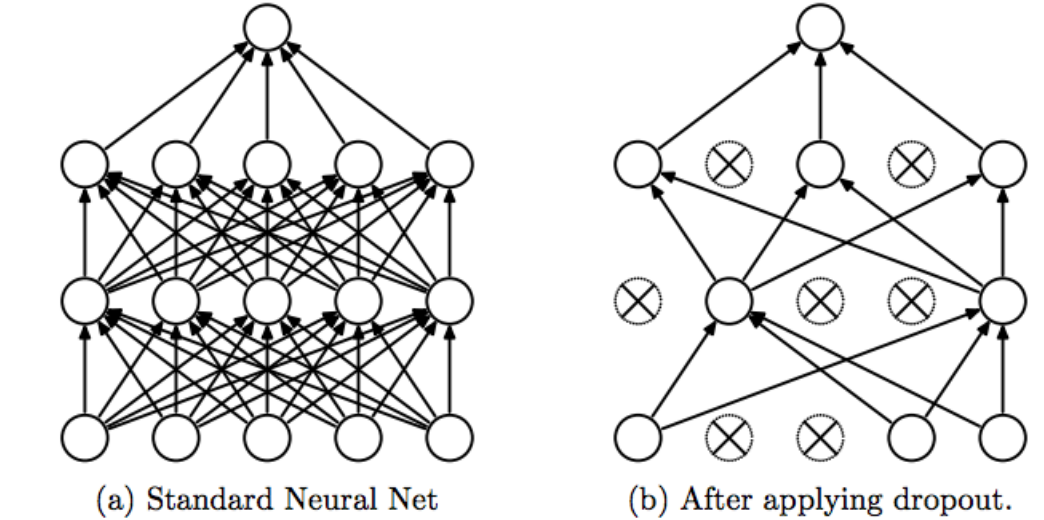
\includegraphics[scale=0.35]{images/dropout.png}
\caption{Dropout Neural Net Model~\parencite{srivastava2014dropout}: Left (a): A standard neural network. Right (b): This is one of the sub-networks. dropout is applied on the standard network shown on the left and the random units are dropped. 
}
    \label{fig:Early_stopping}
\end{figure}

\subsection{Weight decay}

When the training data is simple but the model is highly complex, overfitting occurs as the weights gradually increase during training. The larger the weights, the more it is affected by the training data, and the model fits too perfectly to the seen data. This is a phenomenon in which the model is affected by local noise and becomes fit to outliers. Weight decay is often used to avoid this problem by limiting the increase of weights to reduce the model complexity~\parencite{krogh1992simple}. Weight decay minimises a loss function by including a penalty on the $L_2$ Norm of the weights, and this is described in the following Equation~\ref{eq:weight_decay}:

\begin{equation}
    L_{new}(w) = L_{original}(w) + \lambda w^Tw ,
    \label{eq:weight_decay}
\end{equation}


where $\lambda$ is a regularization parameter determining how to trade off the large weight penalty with the original loss L and $\lambda w^Tw$ is a \textit{regularizer}. Adding this regularizer to the loss function suppresses the weight increase. 
%This is because neural network's learning is based on gradient descent. Since the l2 norm of the weight means the size of the weight parameter, by additionally reflecting a certain ratio of the current weight size to the loss, the weight at the current time is reduced by a certain ratio, and then the gradient calculated from the error is updated.

\section{Related Work}

%The way to preserve confidentiality in deep learning based NLP can have different approach. \parencite{carlini2019secret} This scenario is that a company has the both the right to access the original documents and the neural NLP models. However, when 
%the proposed project, our scenario is that we only can access to the N-grams instead of the whole original data. Therefore, this project can expand the possibility to share confidential data in fragmented format and finally improving neural NLP models. 

% \subsection{Privacy in deep learning}

% As deep learning (DL) advances, the importance of preserving privacy and confidentiality is also emerging. 

% According to \cite{shokri2015privacy}, previous studies on privacy in DL addresses three aspects: 1) privacy of input data for training a model 2) privacy of the model itself 3) privacy of the output of the model. 
% Deep learning systems rely on a massive amount of training data that may include private and sensitive information.

% Therefore, a new approach is required and in this context, \parencite{carlini2019secret} showed neural NLP models can unintentionally memorise the original data and suggested potential defences against it.
%and in this context, \cite{carlini2019secret} showed neural NLP models can unintentionally memorize the original data and suggested potential defenses against it.

\subsection{Using confidential data in NMT}

To our knowledge, the use of confidential data in MT has not received much attention recently. \cite{cancedda-2012-private} proposed an encryption-based (one-time pad) method for phrase-based statistical machine translation (PB-SMT). However, PB-SMT is nowadays clearly outperformed by NMT \parencite{bentivogli-etal-2016-neural}, which function completely differently compared to classical statistical models. Therefore, new solutions are required to preserve data confidentiality. 

In the broader context of NLP, secure multi-party computation~\parencite{feng2020securenlp} and homomorphic encryption~\parencite{al2020privft} have been used to provide strong privacy guarantees. Since these cryptographic methods incur high performance penalties (see~\parencite{riazi2019deep} for an overview of their performance in deep learning), more recent proposals have focused on the careful use of simpler cryptographic primitives while training a model over encrypted text due to confidentiality reasons. For instance, TextHide~\parencite{huang-etal-2020-texthide} allows to perform natural language understanding tasks while requiring the participants to complete an encryption step in a federated setting. 
%However the privacy claims of TextHide are subject to debate~\cite{carliniblog} and the way encryption is used (and the privacy guarantees it provides) in TextHide is at the center of the debate.
%As summarized in Figure~\ref{fig:scenario}, we tackle a different problem in this paper: Is it possible to improve the quality of NMT systems by domain adaptation while preventing the full reconstruction of a natural text document used for training? 
%propose a different approach to achieve confidentiality in NMT by borrowing techniques from NLP itself. 
%\AB{we propose a simpler approach that does not require federated learning setup..?}\ftnote{TLDR: "Better not to dig into this" More: I think this is tricky to state: Federated setting may require the clients to run some encryption code and do local training while here we need the construction of phrase pairs by the clients... If we want to refer to a Trusted Third party concept then there are cryptographic proposals for that as well.}
%
The aforementioned studies are mostly assuming accessibility of the original data, and focus on preventing explicit/implicit leakage of partial information while training the models on such data. 
%However, in many cases, although the original data is essential to improve NLP models including NMT systems, we cannot have the right to access it. 
By contrast to previous studies, the novel approach taken in this thesis work is exploring the possibility of using fragmentation of confidential data for improving state-of-the-art NMT applications. 
%By contrast, we explore the possibility of using fragmented data to improve state-of-the-art NMT applications.
%Moreover, our work paves the way for a further study on the implications of data fragmentation for confidentiality purposes.  %\forFT{ should we mention this? "... and quantifying the trade-off/loss in data usefulness for training NMT models."}

% \section{Privacy Attack}

% It aims to steal personal information buried somewhere in the model.
% At this time, one of the main settings to know is whether the target model is black-box or white-box.
% You can think of the black-box setting as an attack on the MLaaS-type model API like BigML, in which the structure or weight of the model cannot be known at all, and a specific input value is sent to the model (querying inputs) and the result is returned.
% You can think of the white-box setting as a setting that can access both the model's structure and weights, and even training and inference.